\documentclass[letterpaper, 12pt, oneside]{article}%especificaciones del documento
\usepackage{amsmath}%paquete para escribir expresiones matemámaticas
\usepackage{graphicx}%paquete para poder incluír imagenes en el documento
\usepackage{xcolor} %paquete de LaTex para poder poner otro texto
\graphicspath{{Imagenes/}}%directorio de la imagen, este lo cambian por el directorio en el que ustedes guardaron su imagen 1.png
\usepackage[utf8]{inputenc} %para poder poner acentos0

	\title{\Huge Taller de Herramientas Computacionales}
	%\title{\Huge \colorbox{magenta}{Taller de Herramientas computacionales}} %De esta forma con colorbox pone el texto dentro de una "caja" de color.
	\author{Josué Artemio Hernández Rodríguez}%autor del escrito
	\date{09/01/19}%fecha del escrito

\begin{document}%inicia el documento
\maketitle
%\vfill %Para rellenar el espacio y colocar hasta abajo de la pagina el siguiente texto, imagen.
\begin{center}%inicia centrado
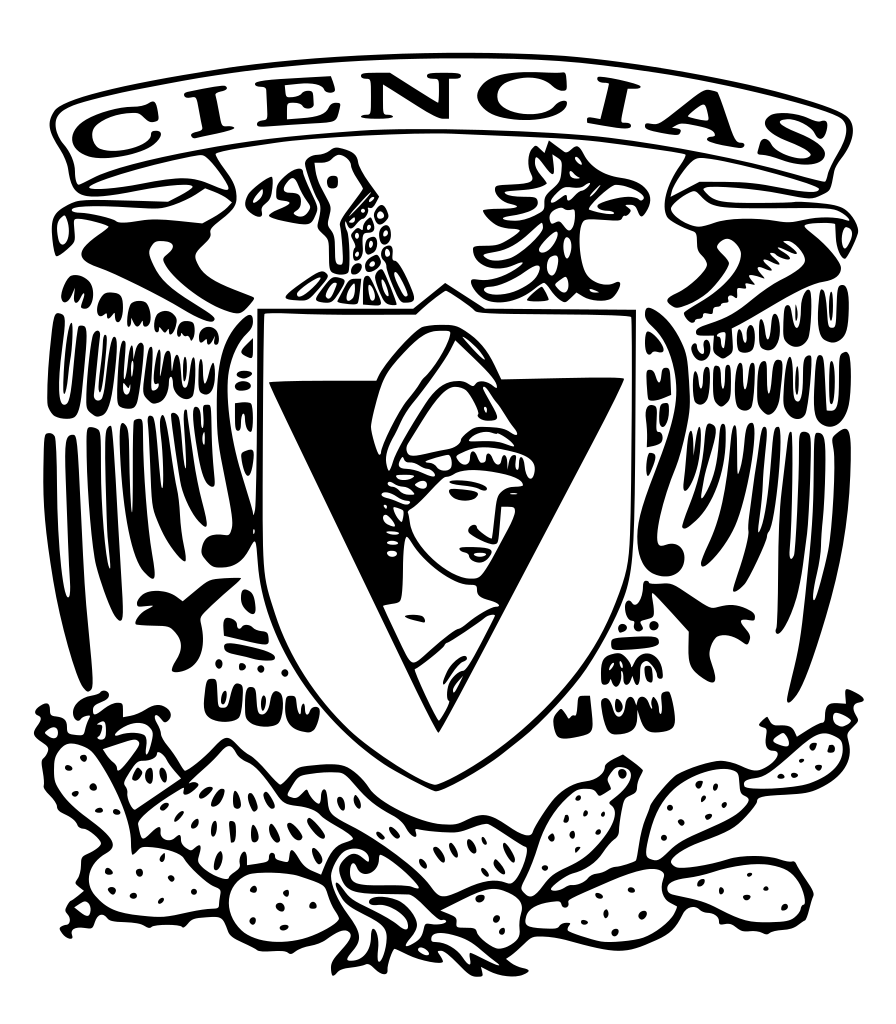
\includegraphics[scale=0.2]{2.png}%del lado izquierdo se muestra el tamaño de la imagen, del derecho se escribe el nombre de la imagen a incluir en el texto
\end{center}%termina el centrado para la imagen
\newpage%crea una nueva página

\title{\Huge Trabajando con git\\}%titulo2 \\ sirven para saltar una linea.

Lo que vimos en clase fue:%letras de color azul
\begin{enumerate}%Inicio de númeración para enlistar las cosas vistas en clase.
	\item Algunos conceptos y software utilizado en clase%item sirve enlistar el elemento, este es el primer elemento enumerado.
		\begin{itemize}
			\item git esta compuesto por un cliente web y otro en modo texto
			\item Un archico o directorio que tiene esta estrcutura ".archivo/" significa que esta oculto
			\item Existen otros editores de texto en linux, como lo son "vi" y "gedit"
			\item Gitlab cumple con la mismas funciones que github, la de tener en la nube tus repositorios
		\end{itemize}
	
	\item Comandos de Bash%Segundo elemento enumerado.
	\begin{itemize}%comienza el enlistado pero itemize a diferencia de enumerate enlista sin un orden secuencial (es decir no utiliza números, ni letras)
		\item "gedit" o "vi" abren los editores de texto correspondintes
		\item cat muestra el contenido de un archivo
		\item mkdir -p: Crea los directorios necesarios para llegar a una ruta deseada
		\item cd lleva a home
		\item git push: para subir informacion a gitub
		\item git pull: para bajar la información de github
		\item history > Clases/Latex/Comandos03.txt:  Guarda el historial de comandos en un archivo llamado Comandos.txt
		
				
	\end{itemize}%finaliza enlistado con itemize
	\item Pasos para resolver un problema eficazmente
		\begin{enumerate}
			\item Problema
			\item Definir (entender)
			\item analizar y delimitar el problema
			\item Soluciones
			\item Describir la solución con detalle
			\item Solución general
		\end{enumerate}
	\item \textbf{Tarea}
	\\
	Buscar un problema de física que requiera la aplicacion de una fórmula para resolverlo
		
	
\end{enumerate}%finaliza el enlistado principal
	


\end{document}%termina el documento